\xpartbox{Near Duplicates Detection}

\begin{xpsectionbox}{Description}{}

The raw data-set contains fairly many duplicate images due to multiple postings of the same photograph. Such duplicates (or near-duplicates) need to be identified and collected in bunches that would be represented by the highest quality images.

\begin{minipage}{0.4\linewidth}

\begin{itemize}
	  \item Haar wavelets computations
	  \item distance measure definition (threshold)
	  \item champion selection (highest resolution)
\end{itemize}
\end{minipage}
\begin{minipage}{0.6\linewidth}

\begin{center}
%			%\hspace{-5cm}
%			\vspace{-1cm}
			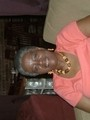
\includegraphics[height=0.25\linewidth]{images/NearDupScaleRot}
			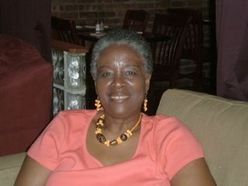
\includegraphics[height=0.25\linewidth]{images/NearDupScale}
\end{center}

\end{minipage}
\end{xpsectionbox}

%\begin{xpsectionbox}{Challenges}{}
%
%\begin{minipage}{0.4\linewidth}
%\begin{itemize}
%	  \item low-quality images
%	  \item various lighting conditions
%	  \item frontal vs. profile faces
%	  \item various skin colors
%	  \item occlusions, facial hair, spectacles, hat, etc.
%\end{itemize}
%\end{minipage}
%\begin{minipage}{0.6\linewidth}
%\begin{center}
%			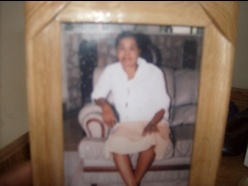
\includegraphics[height=0.25\linewidth]{images/PL_low_quality}
%			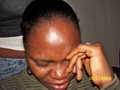
\includegraphics[height=0.25\linewidth]{images/HEPL_occlusion}
%			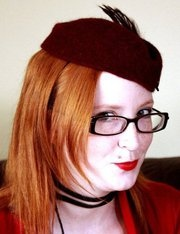
\includegraphics[height=0.25\linewidth]{images/HEPL_spectacles_hat}
%\end{center}
%\end{minipage}
%
%\end{xpsectionbox}
%
%\xpartbox{Solution}
%
%%--------------------------------------------------------------------------------------------------------------------
%\begin{xpsectionbox}{}{}
%
%
%\begin{minipage}{0.5\linewidth}
%\bf{Method:}
%
%\begin{itemize}
%	  \item Haar like features  
%	  \item moving window technique
%	  \item Ada boost classifier cascade
%\end{itemize}
%\begin{center}
%			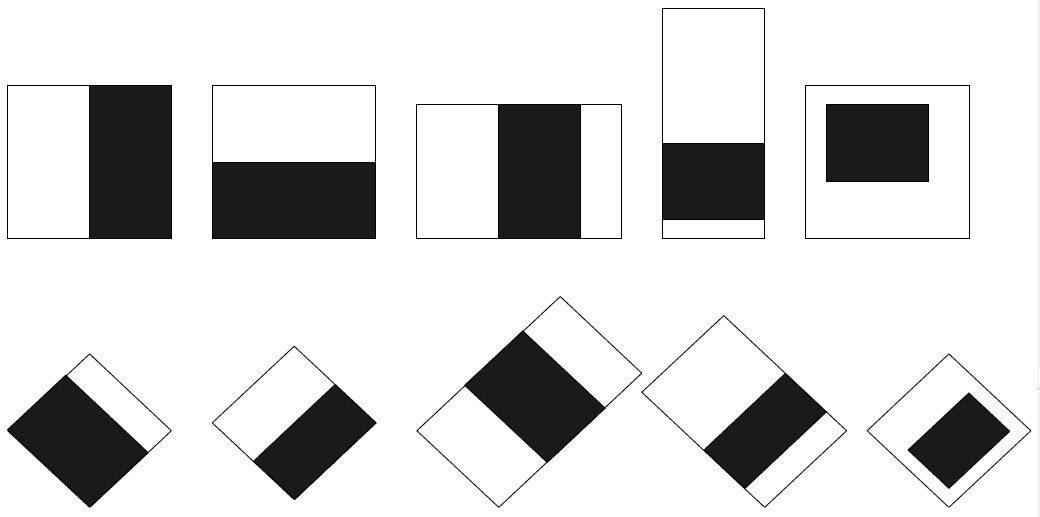
\includegraphics[height=0.25\linewidth]{images/Haar_features}
%\end{center}
%
%\bf{Drawbacks:}
%\begin{itemize}
%	  \item small size faces not detectable
%	  \item lighting/occlusion deteriorates results 
%\end{itemize}
%\begin{center}
%			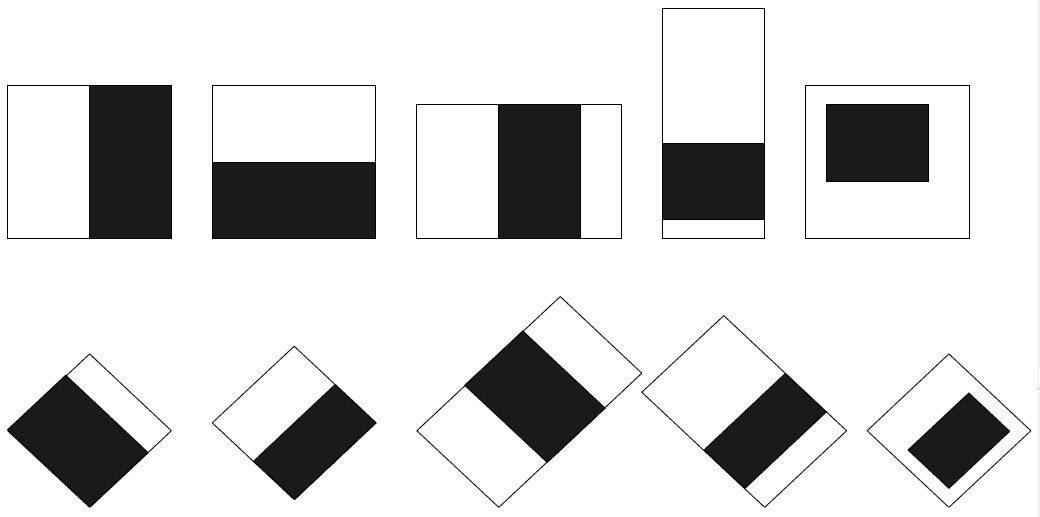
\includegraphics[height=0.25\linewidth]{images/Haar_features}
%\end{center}
%
%\end{minipage}
%\begin{minipage}{0.5\linewidth}
%\bf{Improvements:}
%
%\begin{itemize}
%	  \item color information (skin) 
%	  \item learning color models
%	  \item extended color space + neural network
%\end{itemize}
%\begin{center}
%			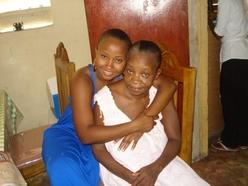
\includegraphics[height=0.2\linewidth]{images/Lena_RGB}
%			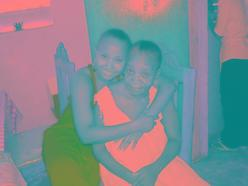
\includegraphics[height=0.2\linewidth]{images/Lena_LAB}
%			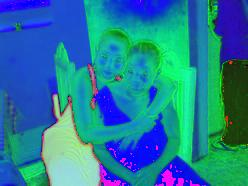
\includegraphics[height=0.2\linewidth]{images/Lena_HSV}
%			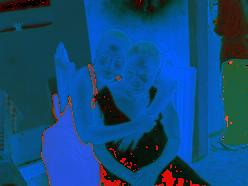
\includegraphics[height=0.2\linewidth]{images/Lena_LUV}
%\end{center}
%\bf{Advantages:}
%\begin{itemize}
%	  \item high precision skin detection(91\%)  
%	  \item skin maps focus the face finding
%	  \item enhance skin region intensities
%\end{itemize}
%\begin{center}
%			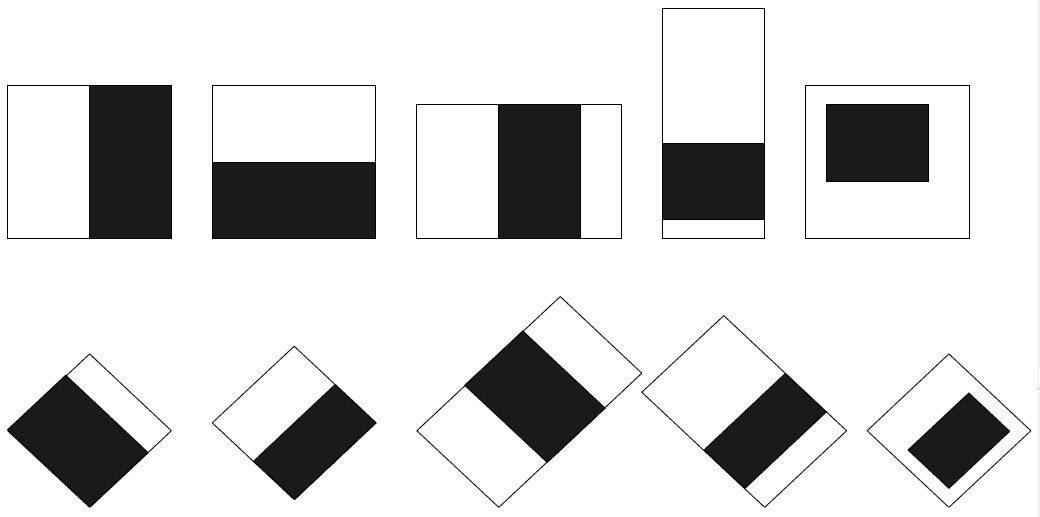
\includegraphics[height=0.2\linewidth]{images/Haar_features}
%\end{center}
%\end{minipage}
%\end{xpsectionbox}

\xpartbox{Experiments}

\begin{xpsectionbox}{Results}{}

\begin{itemize}
	\item Data (HEPL(x), PL(y), AFLW(z))
	\item Difficulties (quality, lighting, occlusion, no annotation, etc.)
	\item Result for HEPL: x\% duplicates
	\item Result for PL: y\% duplicates 
		
\end{itemize}
\end{xpsectionbox}